\documentclass[10pt,a4paper]{article}

\usepackage[margin=0.62in,top=0.55in,bottom=0.62in]{geometry}
\usepackage[T1]{fontenc}
\usepackage{newtxtext,newtxmath}
\usepackage[varqu]{inconsolata}
\usepackage{amsmath}
\usepackage{booktabs}
\usepackage{tabularx}
\usepackage[expansion=false]{microtype}
\usepackage{enumitem}
\usepackage{xurl}
\usepackage[hidelinks]{hyperref}
\usepackage{xcolor}
\usepackage{tikz}
\usetikzlibrary{arrows.meta,positioning,calc}
\usepackage{pgfplots}
\pgfplotsset{compat=1.16}
\usepackage{caption}
\captionsetup{font=footnotesize,labelfont=bf,skip=2pt}
\usepackage{graphicx}

\usepackage{titlesec}
\titlespacing*{\section}{0pt}{9pt}{4pt}
\titlespacing*{\paragraph}{0pt}{2pt}{5pt}
\titleformat*{\section}{\large\bfseries\color{ink}}
\setlength{\textfloatsep}{5pt}
\setlength{\floatsep}{4pt}
\setlength{\intextsep}{4pt}
\setlist{nosep,leftmargin=1.1em}
\setlength{\parskip}{4pt}
\linespread{1.06}
\setlength{\parindent}{0pt}
\setlength{\tabcolsep}{4pt}
\raggedbottom
\setlength{\emergencystretch}{2em}

% ---------- colours ----------
\definecolor{ink}{HTML}{1A365D}
\definecolor{cA}{HTML}{2B6CB0}   % blue
\definecolor{cB}{HTML}{DD6B20}   % orange
\definecolor{cC}{HTML}{2F855A}   % green
\definecolor{cD}{HTML}{805AD5}   % purple
\definecolor{cG}{HTML}{718096}   % grey

\begin{document}

% ---------- Title Page ----------
\begin{titlepage}
\centering
\vspace*{1.2cm}

\IfFileExists{iitd.png}{{\includegraphics[width=4.2cm]{iitd.png}}}{}

\vspace{1.0cm}

{\huge\scshape Indian Institute of Technology Delhi\par}

\vspace{0.4cm}

{\Large COL764: Information Retrieval and Web Search\par}

\vspace{2.2cm}

{\rule{0.85\textwidth}{0.8pt}\par}
\vspace{0.6cm}
{\LARGE\bfseries Assignment 4: Iterative Retrieval for Multi-hop\\[4pt] Question Answering\par}
\vspace{0.6cm}
{\rule{0.85\textwidth}{0.8pt}\par}

\vspace{2.5cm}

{\Large\bfseries Instructor\par}
\vspace{0.25cm}
{\Large Prof.\ Srikanta Bedathur\par}

\vspace{1.2cm}

{\Large\bfseries Submitted by\par}
\vspace{0.25cm}
{\Large Aditya Anand\par}
\vspace{0.1cm}
{\large 2023CS50284\par}

\vfill

{\Large \today\par}

\vspace{1cm}

\end{titlepage}

% =====================================================================
\newpage

\section*{Overview}
A two-hop question names one entity but asks about another that it only describes, the \emph{bridge}. The agent
finds the bridge first, searches again with it, and spends the LLM calls it has left on checking the answer.

\begin{center}
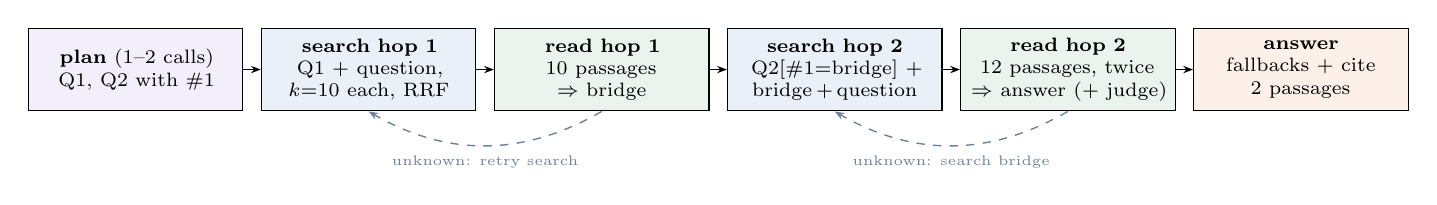
\begin{tikzpicture}[font=\scriptsize, node distance=0.22cm,
  st/.style={draw=black, line width=0.4pt, align=center, text width=2.55cm, inner sep=2.5pt, minimum height=1.05cm},
  arr/.style={-{Stealth[length=3.5pt]}, black, line width=0.5pt}]
  \node[st, fill=cD!10] (p) {\textbf{plan} (1--2 calls)\\Q1, Q2 with \#1};
  \node[st, fill=cA!10, right=of p] (s1) {\textbf{search hop 1}\\Q1 + question, $k{=}10$ each, RRF};
  \node[st, fill=cC!10, right=of s1] (r1) {\textbf{read hop 1}\\10 passages\\$\Rightarrow$ bridge};
  \node[st, fill=cA!10, right=of r1] (s2) {\textbf{search hop 2}\\Q2[\#1=bridge] + bridge\,+\,question};
  \node[st, fill=cC!10, right=of s2] (r2) {\textbf{read hop 2}\\12 passages, twice\\$\Rightarrow$ answer (+ judge)};
  \node[st, fill=cB!10, right=of r2] (a) {\textbf{answer}\\fallbacks + cite 2 passages};
  \foreach \u/\v in {p/s1,s1/r1,r1/s2,s2/r2,r2/a} \draw[arr] (\u) -- (\v);
  \draw[arr, dashed, cG] (r1.south) to[out=-150,in=-30] node[below, font=\tiny]{unknown: retry search} (s1.south);
  \draw[arr, dashed, cG] (r2.south) to[out=-150,in=-30] node[below, font=\tiny]{unknown: search bridge} (s2.south);
\end{tikzpicture}
\end{center}

% =====================================================================
\section{Single-shot vs.\ iterative}
\begin{minipage}[t]{0.585\textwidth}
\vspace{0pt}
\centering\footnotesize
\begin{tabular}{@{}lcccccc@{}}
\toprule
Dev set, 300 questions & EM & Ans.\ F1 & Ev.\ F1 & $S$ & Search & LLM\\
\midrule
B1 single-shot (starter) & 0.1400 & 0.2110 & 0.3717 & 0.2431 & 1.00 & 1.00\\
B2 staff iterative (leaderboard) & 0.2033 & 0.2596 & 0.4767 & 0.3030 & 2.03 & 3.03\\
\textbf{My agent (final)} & \textbf{0.4967} & \textbf{0.5965} & \textbf{0.6650} & \textbf{0.6102} & 4.37 & 5.25\\
\bottomrule
\end{tabular}
\captionof{table}{$S = 0.8\cdot$Ans.\ F1$\,+\,0.2\cdot$Ev.\ F1. Search, LLM: mean calls per question. All 300 questions ran without errors.}
\label{tab:main}
\end{minipage}\hfill
\begin{minipage}[t]{0.395\textwidth}
\vspace{0pt}
\centering\footnotesize
\begin{tabular}{@{}lcc@{}}
\toprule
Diagnostic & B1 & Mine\\
\midrule
both gold paragraphs retrieved & 15.3\% & 69.7\%\\
hop-2 paragraph retrieved & 23.3\% & 72.3\%\\
bridge (hop-1 answer) correct & -- & 76.3\%\\
gold paragraphs cited (of 2) & 0.74 & 1.33\\
\bottomrule
\end{tabular}
\captionof{table}{Retrieval and bridge accuracy (\texttt{dev/analyze.py}).}
\end{minipage}

\smallskip
Iterating lifts exact match from 0.14 to 0.50 and evidence F1 from 0.37 to 0.67. The gain comes from the second
search: B1 retrieves both gold paragraphs for 15\% of questions, the agent for 70\%. Figure~\ref{fig:steps} shows how
dev $S$ grew as the components were added.

\vfill
% =====================================================================
\section{Design}
\textbf{\texttt{next\_query}.} \emph{Split.} One LLM call rewrites the question as Q1 and Q2, where Q2 uses \#1 for
Q1's answer. A plan is asked again if Q2 lacks \#1, if Q1 repeats the question, asks for a date or a number (a
bridge is always an entity) or drops every name in the question. If the retry also fails, a possessive
(\emph{X's team}) or \emph{the Y of X} phrase is split off without the LLM. \emph{Search.} Hop~1 searches with Q1
and with the full question, hop~2 with Q2 (bridge filled in) and with bridge + question. Each search returns 10
passages, and the two lists are merged by reciprocal rank fusion. \emph{Retry.} After a failed read, hop~1 searches
with Q1 plus the first sentence of a passage the LLM writes as a guess (Query2doc); hop~2 searches with the bridge
alone, or for \emph{when} questions with the bridge plus a Query2doc sentence. If hop~1 keeps failing, the bridge
comes from the model's memory.

\textbf{\texttt{should\_stop} and \texttt{answer}.} \emph{Read.} The LLM sees 10 whole passages at hop~1 and 12 at
hop~2. The 4B reader depends on order (Figure~\ref{fig:pos}), so at hop~1 the article the question names goes first,
and a bridge read from a lower passage is checked again after a Query2doc search. \emph{Check.} The hop-2 answer is
read a second time with the passages reversed and the original question; if the answers differ, a judge call picks
one and keeps the first when unsure. A spare call asks for the answer without passages, and the judge compares
again if a passage supports it. In the final run these checks replaced 21 answers, 9 for the better and 1 for the
worse. \emph{Stop.} The loop ends once hop~2 has an answer of the asked type (a date for \emph{when}, a number for
\emph{how many}) that is not the bridge, or when one LLM call or 15\,s is left. \emph{Answer.} If hop~2 never
answered, the model guesses with the bridge as a hint; a rejected hop-2 answer and a span from the best passage are
the fallbacks. The answer is returned as written, with two citations: a passage with the bridge and one with the
answer. If the server fails a call, the agent goes on with its remaining budget; with 5\% of calls failing, $S$ is
0.601 instead of 0.539.
\emph{Did not help:} a third hop-2 search at the start ($S$ $-$0.022, as retries lost their search) and asking for
the answer copied word for word ($-$0.049).

\vfill
\noindent\begin{minipage}[t]{0.485\textwidth}
\centering
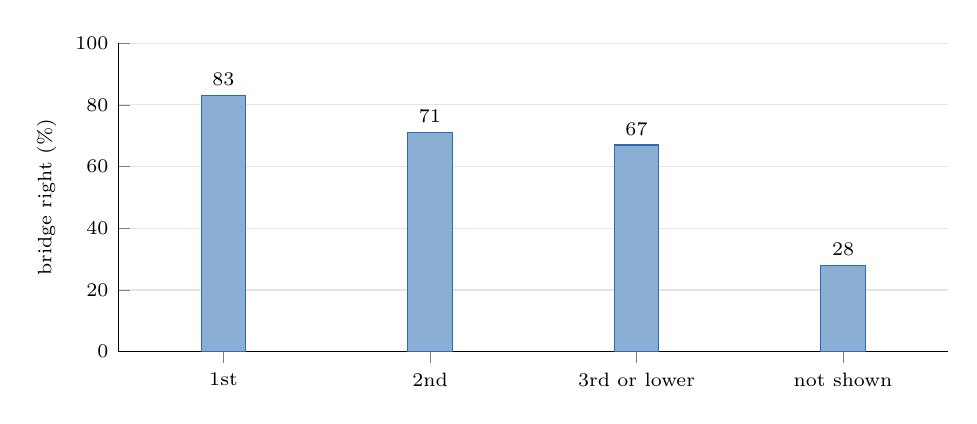
\begin{tikzpicture}
\begin{axis}[ybar, width=\linewidth, height=5.5cm, bar width=16pt, ymin=0, ymax=100, ylabel={bridge right (\%)},
  symbolic x coords={1st,2nd,3rd or lower,not shown}, xtick=data, enlarge x limits=0.17,
  nodes near coords, nodes near coords style={font=\scriptsize}, tick label style={font=\scriptsize}, label style={font=\scriptsize}, axis lines*=left, ymajorgrids, grid style={gray!20}]
\addplot[fill=cA!55, draw=cA] coordinates {(1st,83) (2nd,71) (3rd or lower,67) (not shown,28)};
\end{axis}
\end{tikzpicture}
\captionof{figure}{First hop-1 read: bridge accuracy by where the gold passage was shown ($n$ = 214, 24, 24, 32).}
\label{fig:pos}
\end{minipage}\hfill
\begin{minipage}[t]{0.485\textwidth}
\centering
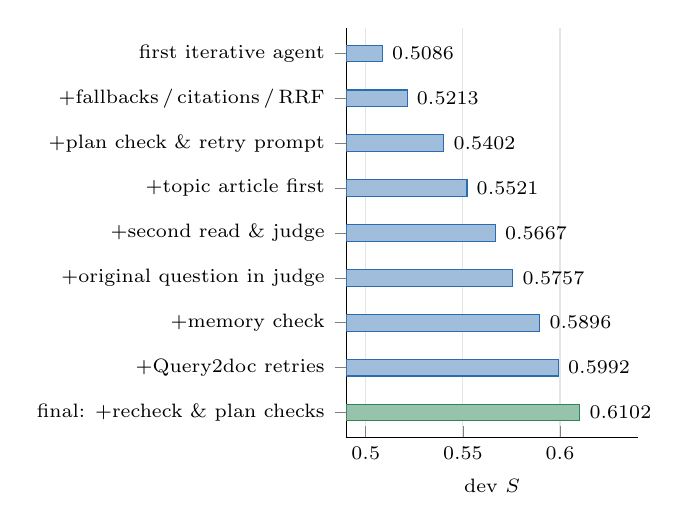
\begin{tikzpicture}
\begin{axis}[xbar, bar shift=0pt, width=3.7cm, height=5.2cm, scale only axis, bar width=6pt,
  xmin=0.49, xmax=0.64, xtick={0.50,0.55,0.60}, xlabel={dev $S$},
  xticklabel style={/pgf/number format/fixed, /pgf/number format/precision=2},
  symbolic y coords={a,b,c,d,e,f,g,h,i}, ytick={a,b,c,d,e,f,g,h,i}, y dir=reverse, enlarge y limits=0.07,
  yticklabels={first iterative agent, +fallbacks\,/\,citations\,/\,RRF, +plan check \& retry prompt,
    +topic article first, +second read \& judge, +original question in judge, +memory check,
    +Query2doc retries, final: +recheck \& plan checks},
  yticklabel style={font=\scriptsize}, xticklabel style={font=\scriptsize},
  label style={font=\scriptsize}, axis lines*=left, xmajorgrids, grid style={gray!20},
  nodes near coords, nodes near coords style={font=\scriptsize, /pgf/number format/fixed,
    /pgf/number format/fixed zerofill, /pgf/number format/precision=4}]
\addplot[fill=cA!45, draw=cA] coordinates {(0.5086,a) (0.5213,b) (0.5402,c) (0.5521,d) (0.5667,e) (0.5757,f)
  (0.5896,g) (0.5992,h)};
\addplot[fill=cC!50, draw=cC] coordinates {(0.6102,i)};
\end{axis}
\end{tikzpicture}
\captionof{figure}{Dev $S$ of selected earlier versions as components were added; the last bar is the final agent.}
\label{fig:steps}
\end{minipage}

\vfill
\newpage
% =====================================================================
\section{Error analysis}
\noindent\begin{minipage}[t]{0.50\textwidth}
\vspace{0pt}
The agent gets EM $=0$ on 151 of the 300 dev questions. Figure~\ref{fig:cats} compares the automatic labels from
\texttt{dev/analyze.py} with B1. Iterating cuts bridge failures (i) from 191 to 35, so reading errors (iii) are now
the largest group: 209 questions reach the last read with both gold paragraphs (B1: 46), and on them answer F1 is
0.74. Many (iv) errors are right answers in another form, such as \emph{August 5, 1940} for \emph{5 August 1940}.
My hand labels for the 10 errors in Table~\ref{tab:err} are (i)~3, (ii)~2, (iii)~2, (iv)~2 and (v)~1; only
Berthelot differs from its automatic label (iii), since both gold paragraphs were retrieved.
\end{minipage}\hfill
\begin{minipage}[t]{0.46\textwidth}
\vspace{0pt}
\centering
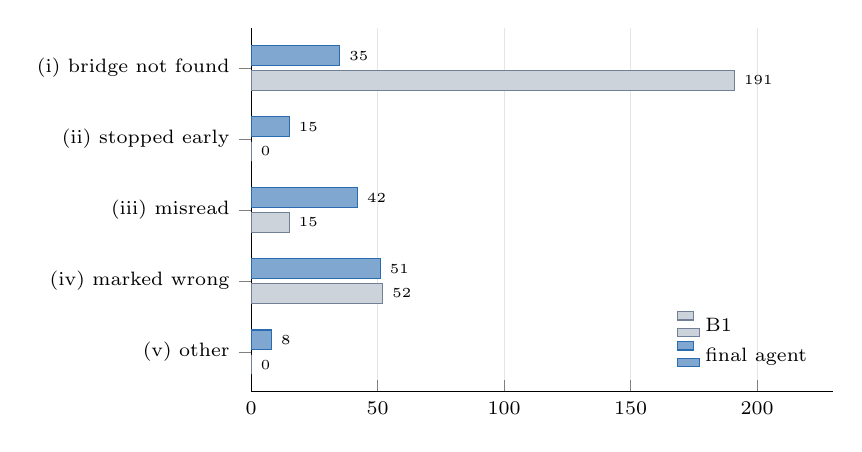
\begin{tikzpicture}
\begin{axis}[xbar, width=0.74\linewidth, height=6.2cm, bar width=7pt, xmin=0, xmax=230,
  symbolic y coords={other,marked,misread,early,bridge}, ytick=data,
  yticklabels={(v) other,(iv) marked wrong,(iii) misread,(ii) stopped early,(i) bridge not found},
  nodes near coords, nodes near coords style={font=\tiny}, enlarge y limits=0.14,
  legend style={font=\scriptsize, at={(0.98,0.04)}, anchor=south east, draw=none, fill=none},
  legend cell align=left, tick label style={font=\scriptsize}, axis lines*=left, xmajorgrids, grid style={gray!20}]
\addplot[fill=cG!35, draw=cG] coordinates {(0,other) (52,marked) (15,misread) (0,early) (191,bridge)};
\addlegendentry{B1}
\addplot[fill=cA!60, draw=cA] coordinates {(8,other) (51,marked) (42,misread) (15,early) (35,bridge)};
\addlegendentry{final agent}
\end{axis}
\end{tikzpicture}
\captionof{figure}{Errors (EM $=0$) by automatic label: B1 258, final agent 151.}
\label{fig:cats}
\end{minipage}

\vfill
\textbf{Example 1 (i), Johnny Berthelot.} The gold paragraph is ranked first, but it says Berthelot sits in the
Louisiana House \emph{based in his hometown of Gonzales}, so the model answers Gonzales; the intended bridge, Baton
Rouge, is only implied. Hop~2 then looks for Auburn wins at Gonzales and guesses 1994, a game played at Auburn
(gold: 1999). With a wrong bridge and no hop-2 paragraph, answer F1 is 0.14 ($n{=}42$), against 0.76 ($n{=}188$)
with the right bridge and paragraph.

\textbf{Example 2 (iii), WAJM.} The bridge and both gold paragraphs are found, but the Atlantic City article has
two undated census paragraphs giving household sizes of 2.50 and 2.46 (gold). The two reads disagree and the judge
keeps the first, 2.50. Nothing in the passages says which census the question means.

\vfill
\begin{center}
\footnotesize\renewcommand{\arraystretch}{1.5}
\begin{tabularx}{\textwidth}{@{}c>{\raggedright\arraybackslash}X>{\raggedright\arraybackslash}p{2.3cm}>{\raggedright\arraybackslash}p{2.6cm}>{\raggedright\arraybackslash}p{3.9cm}@{}}
\toprule
& Question (shortened) & Gold & Mine & What went wrong\\
\midrule
(i) & Last time Auburn won in the work location of Johnny Berthelot? & 1999 & 1994 & bridge \emph{Gonzales} (hometown), not \emph{Baton Rouge}\\
(i) & Sibling of the composer of \emph{Downtown}? & Astrid Young & Michael Gore & bridge \emph{Luke Laird}, writer of Lady Antebellum's \emph{Downtown}, not Neil Young\\
(i) & When did the civil war start in the country Ita Ford is from? & October 15, 1979 & April 1861 & bridge \emph{United States} (her nationality), not El Salvador\\
(ii) & Manager when Tommy Logan's team won the Champions League? & Roberto Di Matteo & Jos\'e Mourinho & bridge Chelsea right; stopped with a search left, hop-2 paragraph never retrieved\\
(ii) & When did Harrysong's country become a member of OPEC? & 1971 & the 1970s & bridge Nigeria right; vague answer accepted, OPEC table never retrieved\\
(iii) & Where did the 2007 World Series winner get Brandon Phillips from? & Los Angeles Angels & Cleveland Indians & both gold paragraphs retrieved, wrong team read\\
(iii) & Average household size in the city served by WAJM? & 2.46 & 2.50 & second read found 2.46; the judge kept 2.50\\
(iv) & When did the country of Saldus Municipality join the Soviet Union? & 5 August 1940 & August 5, 1940 & same date, other order (F1 1.0, EM 0)\\
(iv) & Forest by the southern border of Jerzy Passendorfer's death city? & Kabaty & Kabaty Forest & correct despite a wrong bridge (\emph{Skolim\'ow}); extra word (F1 0.67)\\
(v) & Who was targeted for defrauding the electoral process, in Hotel Courtland's state? & a whole sentence & John Kerry & gold answer is a sentence; hop-2 paragraph never retrieved\\
\bottomrule
\end{tabularx}
\captionof{table}{Ten errors of the final agent, labelled by hand from their traces.}
\label{tab:err}
\end{center}

\vfill
% =====================================================================
\section{AI-use disclosure and code provenance}
I used Claude Code (Anthropic, Claude Opus 5.5) as an assistant throughout this assignment: to understand the
starter code, to implement and debug the agent and the analysis scripts in \texttt{dev/}, to run the experiments, and
to help write and edit this report. I chose which ideas to try and which to keep, checked the results and the
numbers reported here, and take full responsibility for the submission. No external code was copied. The loop follows IRCoT (Trivedi et
al., ACL 2023) and ReAct (Yao et al., ICLR 2023), reciprocal rank fusion follows Cormack, Clarke and Buettcher
(SIGIR 2009), and the data is MuSiQue (Trivedi et al., TACL 2022). BM25, the tools and the scorer come from the
course's \texttt{a4} package. The few-shot examples were written by hand and contain no answers. The agent stores
no answers or data and never recognises a question.

\end{document}
